\documentclass[aspectratio=169]{beamer}

%
% Choose how your presentation looks.
%
% For more themes, color themes and font themes, see:
% http://deic.uab.es/~iblanes/beamer_gallery/index_by_theme.html
%
\mode<presentation>
{
  \usetheme{Madrid}      % or try Darmstadt, Madrid, Warsaw, ...
  \usecolortheme{default} % or try albatross, beaver, crane, ...
  \usefonttheme{default}  % or try serif, structurebold, ...
  \setbeamertemplate{navigation symbols}{}
  \setbeamertemplate{caption}[numbered]
}


\usepackage[T2A]{fontenc}
\usepackage[utf8]{inputenc}
\usepackage[russian]{babel}
\usepackage{stmaryrd}
\usepackage{color, colortbl}
\usepackage{tikz}
\usepackage{caption}


\PassOptionsToPackage{table}{xcolor}
\definecolor{RowColorOdd}{rgb}{0.914,0.914,0.953}
\definecolor{RowColorEven}{rgb}{1,1,1}

\newcommand\myeq{\mathrel{\stackrel{\makebox[0pt]{\mbox{\normalfont\tiny def}}}{=}}}
\newcommand\mywedge{\mathrel{\stackrel{\makebox[0pt]{\mbox{\normalfont\tiny +}}}{\wedge}}}
\newcommand{\specialcell}[2][c]{%
  \begin{tabular}[#1]{@{}c@{}}#2\end{tabular}}

\newcommand{\quot}[1]{«#1»}

\AtBeginSection[]
{
    \begin{frame}
        \frametitle{Содержание}
        \tableofcontents[currentsection]
    \end{frame}
}

\newcommand{\drive}
{
\begin{figure}[t]
\centering
\begin{tikzpicture}[scale=1.5]
% \draw[draw=black, rounded corners=20pt] (0,0) rectangle (5,3);
\draw (0,0) ellipse (16pt and 8pt);
\draw (0,0) node {a};
\draw (-1, 0) node {b};
\end{tikzpicture}
\end{figure}
}

\newcommand{\organization}
{
\begin{figure}[t]
\centering
\begin{tikzpicture}[scale=1.5]
\draw (0,0) node {Задачи СХД};
\draw (-3,0) -- (-1,0);
\draw (3,0) -- (1,0);
\draw (-3,0) [-stealth]-- (-3, -0.85);
\draw (3,0) [-stealth]-- (3, -0.85)
\draw (-3,-1) node {Доступность};
\draw (3,-1) node {Надежность};
\draw (0, -1) node {Производительность};
\draw (0, -0.2) [-stealth]-- (0, -0.85);
\end{tikzpicture}
\end{figure}
}

\newcommand{\dma}
{
\begin{figure}[t]
\centering
\begin{tikzpicture}[scale=.6]
\draw (0, 1) node {CPU};
\draw (0, -2) node {RAM};
\draw (0, -5) node {Block device};

\draw (-2.1, -4.3) rectangle (2.1, -5.7);
\draw (-2.1, -1.3) rectangle (2.1, -2.7);
\draw (-2.1, 1.7) rectangle (2.1, 0.3);


\draw (-1.3, -4.3) [-stealth]-- (-1.3,-2.7);
\draw (1.3, -4.3) [stealth-]-- (1.3,-2.7);

\draw (-1.3, -1.3) [-stealth]-- (-1.3, 0.3);
\draw (1.3, -1.3) [stealth-]-- (1.3, 0.3);
\end{tikzpicture}
\end{figure}
}

\newcommand{\nas}
{
\begin{figure}[t]
\centering
\begin{tikzpicture}[scale=.4]

\draw (-2.3, 2) rectangle (2.3, -6);
\draw (0, 1) node {CPU};
\draw (0, -2) node {RAM};
\draw (0, -5) node {Blk dev};
\draw (0, -6.7) node {Storage Node};

\draw (-2.1, -4.3) rectangle (2.1, -5.7);
\draw (-2.1, -1.3) rectangle (2.1, -2.7);
\draw (-2.1, 1.7) rectangle (2.1, 0.3);
\draw (-1.3, -4.3) [-stealth]-- (-1.3,-2.7);
\draw (1.3, -4.3) [stealth-]-- (1.3,-2.7);
\draw (-1.3, -1.3) [-stealth]-- (-1.3, 0.3);
\draw (1.3, -1.3) [stealth-]-- (1.3, 0.3);

\draw (2.3, -2) [stealth-]-- (4, -2);
\draw (2.3, -2) [-stealth]-- (4, -2);
\draw (6, -2) node {Network};
\draw (4, -1) rectangle (8 ,-3);

\draw (12, 0) node {User};
\draw (10.8, 0.6) rectangle (13.2, -0.6);
\draw (12, -4) node {User};
\draw (10.8, -3.4) rectangle (13.2, -4.6);

\draw (8, -1.8) [stealth-]-- (10.8, 0);
\draw (8, -1.8) [-stealth]-- (10.8, 0);

\draw (8, -2.2) [stealth-]-- (10.8, -4);
\draw (8, -2.2) [-stealth]-- (10.8, -4);

\end{tikzpicture}
\end{figure}
}

\newcommand{\bottleneck}
{
\begin{figure}[t]
\centering
\begin{tikzpicture}[scale=0.5]

\draw (0,0) [stealth-] -- (0, 13);

\draw (-0.5, 10) -- (0.5, 10);
\draw (-2.5, 10) node {\tiny 1999~г. SSE};

\node[align=left, anchor=west] at (1,11.5) 
    {CPU слабые и плохо справляются с логикой СХД\\ Логика СХД выносится в отдельный аппаратный контроллер \\(RAID-контроллер)};

\draw (-0.5, 5) -- (0.5, 5);
\draw (-2.5, 5) node {\tiny 2011~г. NVMe};

\node[align=left, anchor=west] at (1,7.5) 
    {На CPU появляются и развиваются векторные регистры \\ Бутылочным горлышком становится скорость операций с дисками \\ Логика на CPU позволяет внедрять дополнительную функциональность,\\ в том числе увеличивающую скорость операций};

\node[align=left, anchor=west] at (1,2.5) 
    {Появляются более быстрые диски и задачи в индустрии, для которых \\
    они необходимы (например запись видео высокого разрешения)\\
    Логика на CPU тормозит\\
    Ответ --- DPU (data processing unit)
    };



\end{tikzpicture}
\end{figure}
}

\newcommand{\stripe}
{
\begin{figure}[t]
\centering
\begin{tikzpicture}[scale=0.7]

\draw (0,0) rectangle (2,1);
\draw (2,0) rectangle (4,1);
\draw (5,0.5) node {$\ldots$};
\draw (6,0) rectangle (8,1);
\draw (8,0) rectangle (10,1);
\draw (10,0) rectangle (12,1);

\draw (1,0.5) node {$D_0$};
\draw (3,0.5) node {$D_1$};
\draw (7,0.5) node {$D_{N-1}$};
\draw (9,0.5) node {$P$};
\draw (11,0.5) node {$Q$};

\end{tikzpicture}
\captionsetup{labelformat=empty}
\caption{Страйп RAID 6}
\end{figure}
}

\tikzset{radiation/.style={{decorate,decoration={expanding waves,angle=90,segment length=4pt}}},
         disk/.pic={
        code={\tikzset{scale=7/10}
            \draw (1,1) ellipse (1cm and 0.5cm);
            \draw (0,0) arc (180:360:1cm and 0.5cm);%
            \draw (0,-1) arc (180:360:1cm and 0.5cm);%
            \draw (0,-2) arc (180:360:1cm and 0.5cm);%
            \draw (0,-3) arc (180:360:1cm and 0.5cm);%
            
            \draw (0,1) -- (0,-3.05);
            \draw (2,1) -- (2,-3.05);
            \draw (1,1) -- (1,2);
  }}
}

\newcommand{\raid}
{
\begin{figure}[t]
\centering
\begin{tikzpicture}

\path (0,0) pic {disk};
\path (2,0) pic {disk};
\draw (0.7,1.4) -- (2.7,1.4);
\draw (1.7 ,1.7) node {RAID 1};
\draw (0.7,0) node {$A_1$};
\draw (2.7,0) node {$A_1$};

\draw (0.7,-0.7) node {$B_1$};
\draw (2.7,-0.7) node {$B_1$};

\draw (0.7,-1.4) node {$C_1$};
\draw (2.7,-1.4) node {$C_1$};

\draw (0.7,-2.1) node {$\ldots$};
\draw (2.7,-2.1) node {$\ldots$};


\path (6,0) pic {disk};
\path (8,0) pic {disk};
\path (10,0) pic {disk};
\path (12,0) pic {disk};
\draw (6.7,1.4) -- (12.7,1.4);
\draw (9.7 ,1.7) node {RAID 5};


\draw (6.7,0) node {$A_1$};
\draw (8.7,0) node {$A_2$};
\draw (10.7,0) node {$A_3$};
\draw (12.7,0) node {$P_A$};

\draw (6.7,-0.7) node {$B_1$};
\draw (8.7,-0.7) node {$B_2$};
\draw (10.7,-0.7) node {$P_B$};
\draw (12.7,-0.7) node {$B_3$};

\draw (6.7,-1.4) node {$C_1$};
\draw (8.7,-1.4) node {$P_C$};
\draw (10.7,-1.4) node {$C_2$};
\draw (12.7,-1.4) node {$C_3$};

\draw (6.7,-2.1) node {$\ldots$};
\draw (8.7,-2.1) node {$\ldots$};
\draw (10.7,-2.1) node {$\ldots$};
\draw (12.7,-2.1) node {$\ldots$};

\end{tikzpicture}

\end{figure}
}


\newcommand{\raidPerf}
{
\begin{figure}[t]
\centering
\begin{tikzpicture}

\path (0,0) pic {disk};
\path (2,0) pic {disk};
\draw (0.7,1.4) -- (2.7,1.4);
\draw (1.7 ,1.7) node {RAID 1};
\draw (1.7 ,-3) node {Зеркалирование, может ускорять чтение};
\draw (0.7,0) node {$A_1$};
\draw (2.7,0) node {$A_1$};

\draw (0.7,-0.7) node {$B_1$};
\draw (2.7,-0.7) node {$B_1$};

\draw (0.7,-1.4) node {$C_1$};
\draw (2.7,-1.4) node {$C_1$};

\draw (0.7,-2.1) node {$\ldots$};
\draw (2.7,-2.1) node {$\ldots$};


\path (6,0) pic {disk};
\path (8,0) pic {disk};
\path (10,0) pic {disk};
\path (12,0) pic {disk};
\draw (6.7,1.4) -- (12.7,1.4);
\draw (9.7 ,1.7) node {RAID 0};
\draw (9.7 ,-3) node {Страйпинг, ускоряет чтение и запись};


\draw (6.7,0) node {$A_1$};
\draw (8.7,0) node {$A_2$};
\draw (10.7,0) node {$A_3$};
\draw (12.7,0) node {$A_4$};

\draw (6.7,-0.7) node {$B_1$};
\draw (8.7,-0.7) node {$B_2$};
\draw (10.7,-0.7) node {$B_3$};
\draw (12.7,-0.7) node {$B_4$};

\draw (6.7,-1.4) node {$C_1$};
\draw (8.7,-1.4) node {$C_2$};
\draw (10.7,-1.4) node {$C_3$};
\draw (12.7,-1.4) node {$C_4$};

\draw (6.7,-2.1) node {$\ldots$};
\draw (8.7,-2.1) node {$\ldots$};
\draw (10.7,-2.1) node {$\ldots$};
\draw (12.7,-2.1) node {$\ldots$};

\end{tikzpicture}

\end{figure}
}

\newcommand{\writehole}
{
\begin{figure}[t]
\centering
\begin{tikzpicture}[scale=0.5]

% \draw (0,0) rectangle (20,1);

\draw (0,0) rectangle (3.1,1);
\draw (1.55, -0.85) node {$D_1$};
\draw (1.55,1.2) [stealth-]-- (1.55, 2.5);
\draw[align=left, anchor=west] (1.6,2) node {Запись};

\draw[fill=green] (0.1,0.1) rectangle (0.3,0.9);
\draw[fill=green] (0.4,0.1) rectangle (0.6,0.9);
\draw[fill=green] (0.7,0.1) rectangle (0.9,0.9);
\draw[fill=green] (1,0.1) rectangle (1.2,0.9);
\draw(1.3,0.1) rectangle (1.5,0.9);
\draw (1.6,0.1) rectangle (1.8,0.9);
\draw (1.9,0.1) rectangle (2.1,0.9);
\draw (2.2,0.1) rectangle (2.4,0.9);
\draw (2.5,0.1) rectangle (2.7,0.9);
\draw (2.8,0.1) rectangle (3,0.9);

\draw (3.4, 0) rectangle (6.5,1);
\draw (4.95, -0.85) node {$D_2$};
\draw (4.95,1.2) [stealth-]-- (4.95, 2.5);
\draw[align=left, anchor=west] (5,2) node {Запись};


\draw[fill=green] (3.5,0.1) rectangle (3.7,0.9);
\draw[fill=green] (3.8,0.1) rectangle (4,0.9);
\draw[fill=green] (4.1,0.1) rectangle (4.3,0.9);
\draw[fill=green](4.4,0.1) rectangle (4.6,0.9);
\draw[fill=green] (4.7,0.1) rectangle (4.9,0.9);
\draw[fill=green] (5,0.1) rectangle (5.2,0.9);
\draw[fill=green] (5.3,0.1) rectangle (5.5,0.9);
\draw[fill=green] (5.6,0.1) rectangle (5.8,0.9);
\draw[fill=green] (5.9,0.1) rectangle (6.1,0.9);
\draw[fill=green] (6.2,0.1) rectangle (6.4,0.9);

% \draw (3.4, 0) rectangle (6.5,1);
\draw (6.8, 0) rectangle (9.9,1);
\draw (8.35, -0.85) node {$D_3$};


\draw (10.3,0) rectangle (13.4, 1);
\draw (11.85,1.2) [stealth-]-- (11.85, 2.5);
\draw[align=left, anchor=west] (11.9,2) node {Запись};
\draw (11.85,-0.85) node {$P$};
\draw[fill=green] (10.4,0.1) rectangle (10.6, 0.9);
\draw (10.7,0.1) rectangle (10.9, 0.9);
\draw (11,0.1) rectangle (11.2, 0.9);
\draw (11.3,0.1) rectangle (11.5, 0.9);
\draw (11.6,0.1) rectangle (11.8, 0.9);
\draw (11.9,0.1) rectangle (12.1, 0.9);
\draw (12.2,0.1) rectangle (12.4, 0.9);
\draw (12.5,0.1) rectangle (12.7, 0.9);
\draw (12.8,0.1) rectangle (13, 0.9);
\draw (13.1,0.1) rectangle (13.3, 0.9);


\end{tikzpicture}

\end{figure}
}

\newcommand{\san}
{
\begin{figure}[t]
\centering
\begin{tikzpicture}[scale=0.8]


% \draw (1, 0.5) node {Network}; 



\draw (3.25, 1.75) rectangle (5.25, 0.75);
\draw (4.25, 1.225) node {Node};

\draw (3.25, -0.75) rectangle (5.25, 0.25);
\draw (4.25, -0.225) node {Node};

% NAS
\draw (7, 0) rectangle (9, 1);
\draw (8, 0.5) node {Drives}; 
\draw[dashed] (5.8, -0.7) rectangle (9.2, 1.7);
\draw[anchor=south east] (9.1,-0.7) node {\tiny NAS};

% \draw (3,-5) rectangle (8,-2);



% \draw (3,-1) rectangle (8,2);

\draw (3.25, 3) rectangle (6.75, 4);
\draw (5, 3.5) node {Storage Node};

% \draw () elipse
\draw[dashed] (6.225,1.425) ellipse (130pt and 120pt);
\draw[fill=white] (1.5, -0.575) rectangle (2,3.425);
\node[rotate=90] (Nw) at (1.75, 1.425) {Network};

\node[draw] (u1) at (-1,0) {User};
\node[draw] at (-1,1.425) {User};
\node[draw] at (-1,2.85) {User};

%user- - nw
\draw (-0.4, 2.85) -- (1.5, 2.55);
\draw (-0.4, 1.425) -- (1.5, 1.425);
\draw (-0.4, 0) -- (1.5, 0.3);


\draw (5.25, -0.225) -- (7, 0.5);
\draw (5.25, 1.225) -- (7, 0.5);

\draw (3.25, -0.225) -- (2, 0.25);
\draw (3.25, 1.225) -- (2, 1.225);

\draw (3.25, 3.5) -- (2, 2.5);

\end{tikzpicture}

\end{figure}
}


\title[7 июля 2023~г.]{Системы хранения данных}
\author[Васенина А.И.]{Васенина Анна Игоревна}
% \institute[]{Санкт-Петербургский государственный университет \\ Кафедра системного программирования}
\date[]{07 июля 2023~г.}

\newenvironment{comment}{}{}


\begin{document}

\begin{frame}
  \titlepage
\end{frame}

\section{Определение системы хранения данных}

\begin{frame}{СХД и где они обитают}

    \begin{minipage}{0.7\linewidth}
    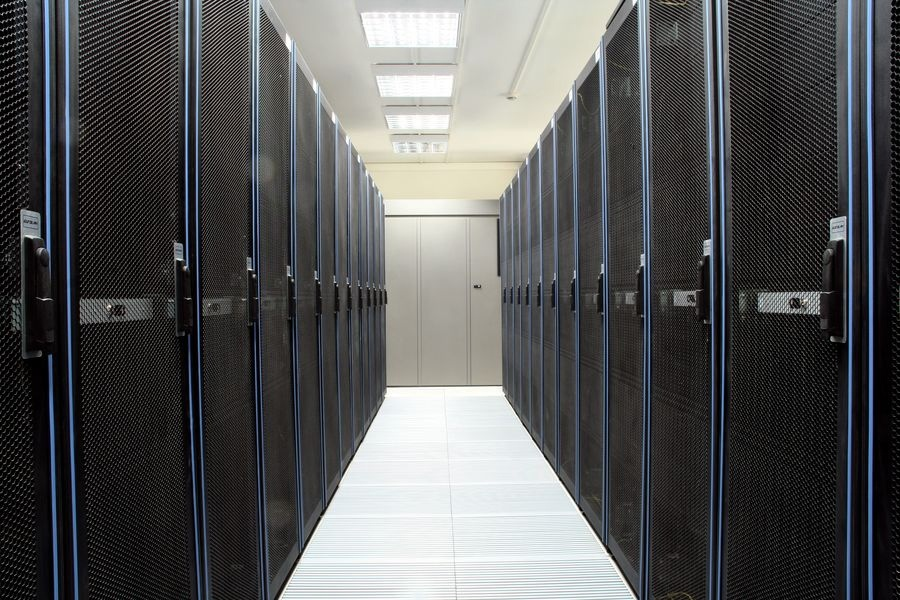
\includegraphics[scale=0.3]{fig/1.servers.jpg}
    \end{minipage}
    \begin{minipage}{0.25\linewidth}
    \vspace{-8em}
    \tiny{\textit{Горный Китай, монастырь Чжоан-Чжоу, год от Рождества Христова 2004-ый. Некто спросил Лин Цзы, что есть мать. И мастер ответил: «Северный и южный мосты есть мать. И шина есть мать. И ещё два десятка конденсаторов есть мать. И много чего ещё есть мать»}}

    \pause
    \vspace{4em}
    \normalsize Так же и с СХД. Очень много чего есть СХД
    \end{minipage}
\end{frame}

\begin{frame}{Неформальное определение СХД}
    \begin{columns}[T] % align columns
    \begin{column}{.48\textwidth}
    \color{red}\rule{\linewidth}{4pt}
    
    Нет!
    \begin{itemize}
        \item Файловая система
        \item База данных
    \end{itemize}
    \end{column}%
    \hfill%
    \begin{column}{.48\textwidth}
    \color{blue}\rule{\linewidth}{4pt}
    
    Да!
    \begin{itemize}
        \item Сложно организованное блочное устройство
    \end{itemize}
    
    \color{black}
    \vspace{4em}
    Блочное ???

    Сложно организованное ???
    \end{column}%
    \end{columns}
        
    
    % \begin{minipage}{0.51\linewidth}
    %     Нет:
    %     \begin{itemize}
    %     \item файловая система;
    %     \item база данных.
    %     \end{itemize}
    % \end{minipage}

    % \begin{minipage}{0.48\linewidth}
    %     Да:
    %     \begin{itemize}
    %     \item сложно организованное блочное устройство.
    %     \end{itemize}


    % \end{minipage}

\end{frame}

\begin{frame}{Блочное устройство}
\begin{columns}
    \begin{column}{.4\textwidth}
        \begin{itemize}
            \item Случайный доступ
            \item Чтение и запись блоками
            \item Блок фиксированного размера
            \begin{itemize}
                \item 512 B
                \item 4 KiB
            \end{itemize}
            \item На современных устройствах большой объем данных
            \item Работа через оперативную память (DMA --- direct memory access)
        \end{itemize}
    \end{column}
    
    \begin{column}{.3\textwidth}
        \dma
    \end{column}
    
    \begin{column}{.25\textwidth}
            \begin{center}
            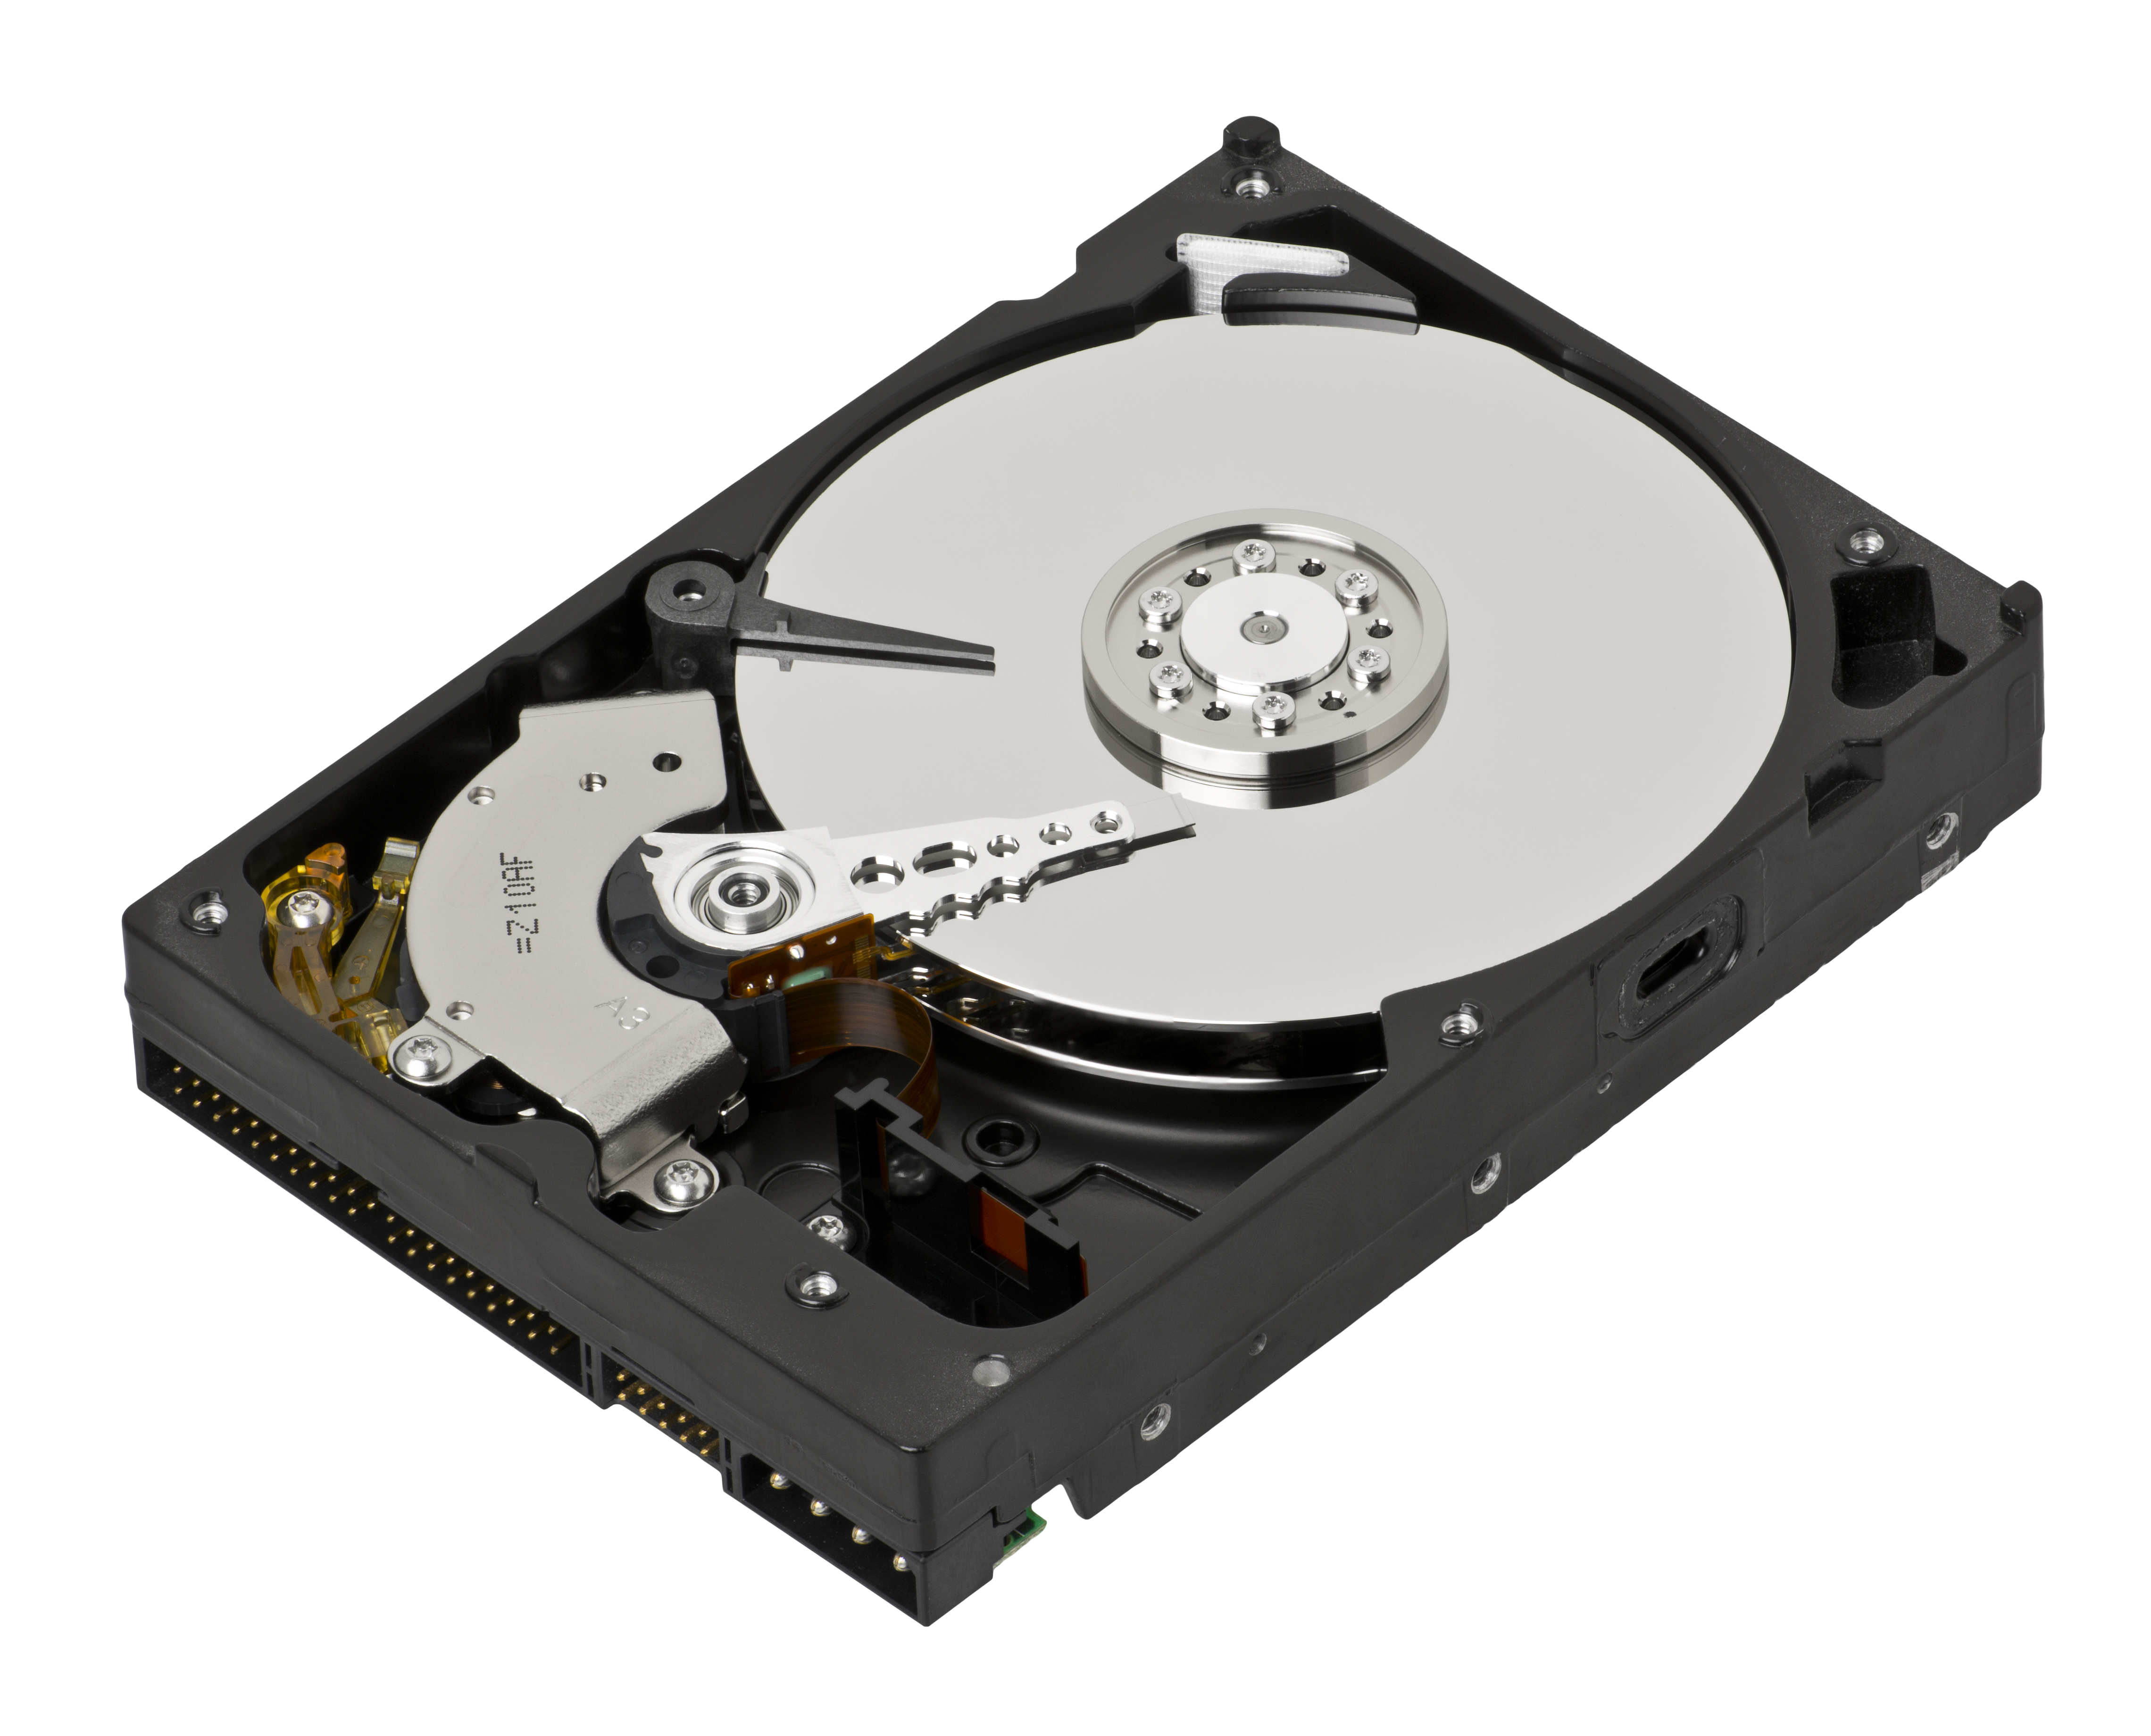
\includegraphics[scale=0.07]{fig/6.hdd.jpg}
            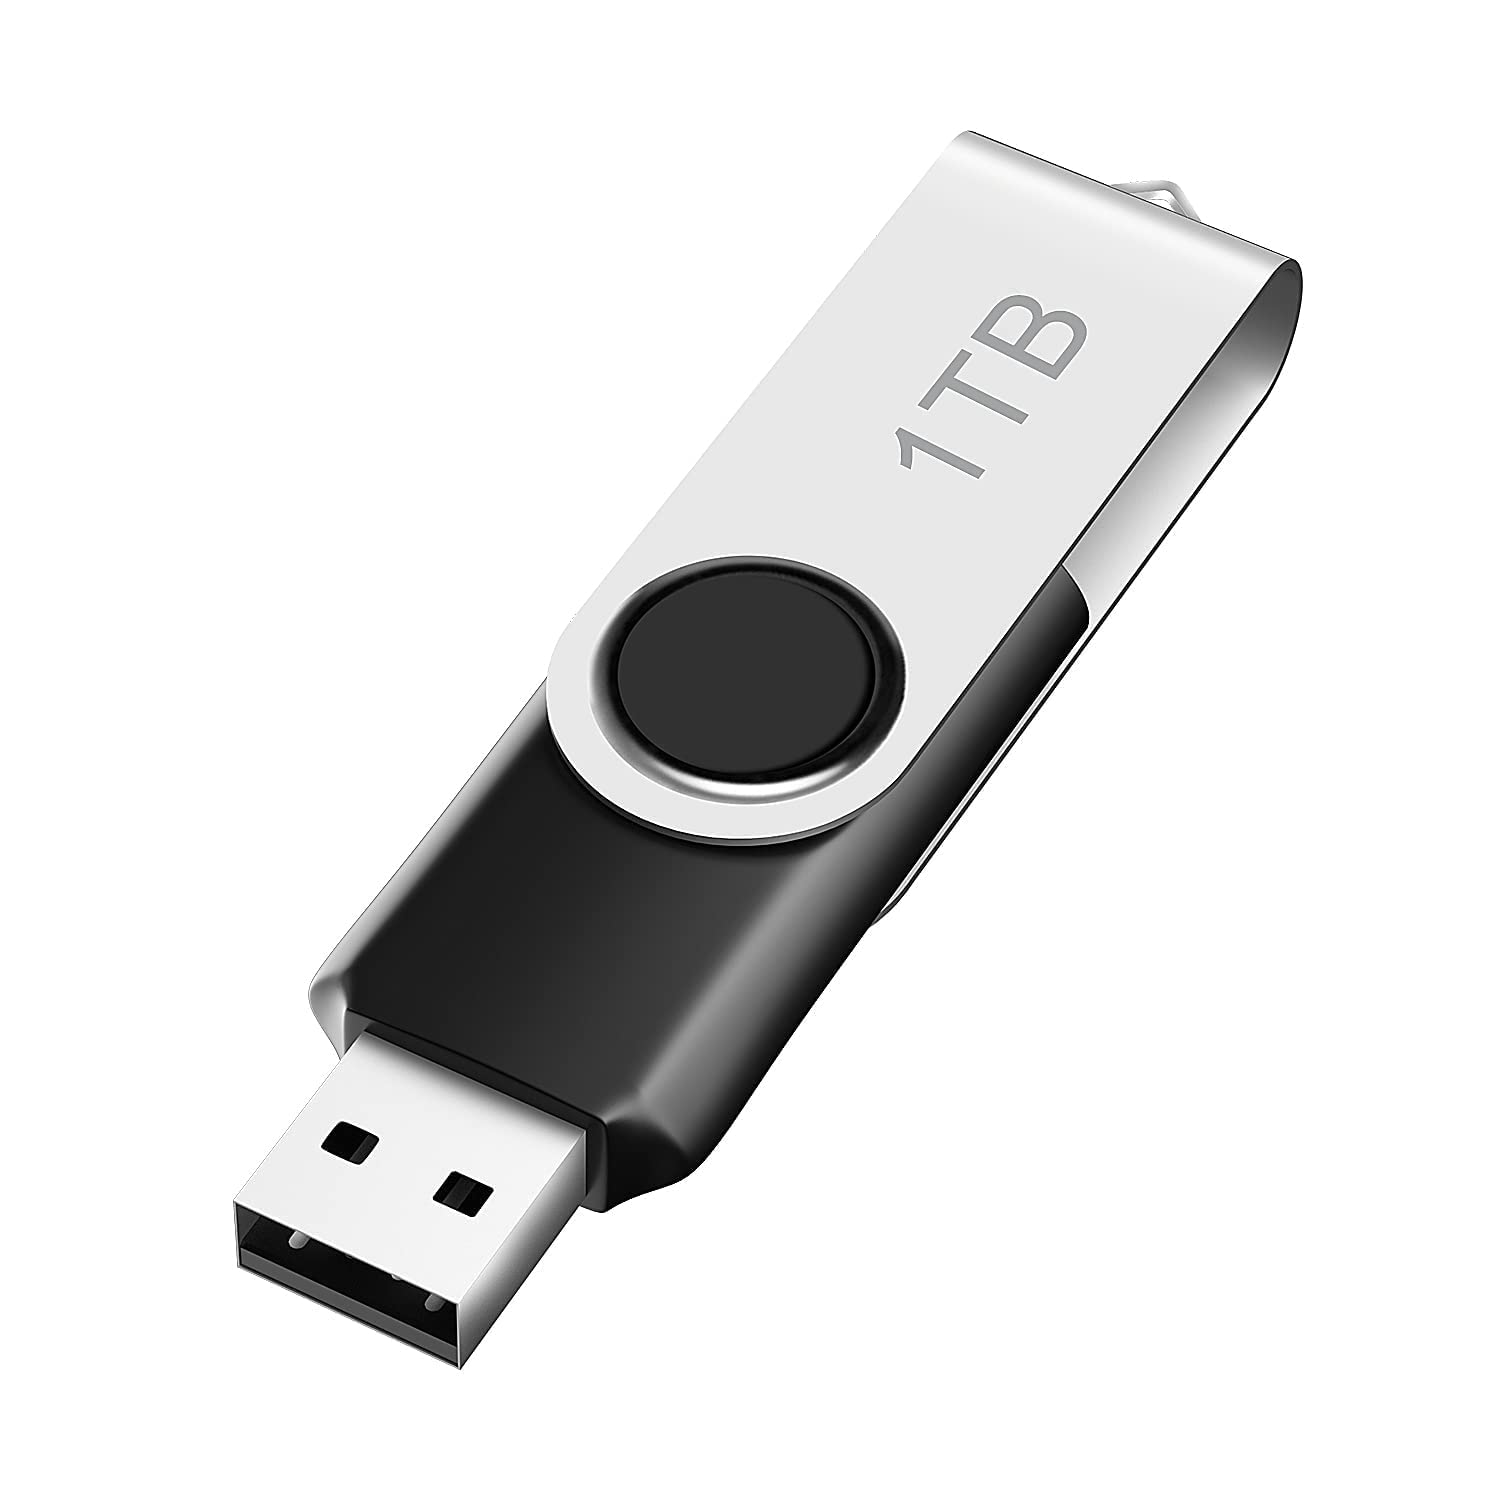
\includegraphics[scale=0.06]{fig/7.flash.jpg}
            \end{center}
            
    \end{column}
\end{columns}
    
    
\end{frame}

\begin{frame}{Сложная организация}
    \organization
\end{frame}

\section{Доступность}

\begin{frame}{Доступность}
    \centering
    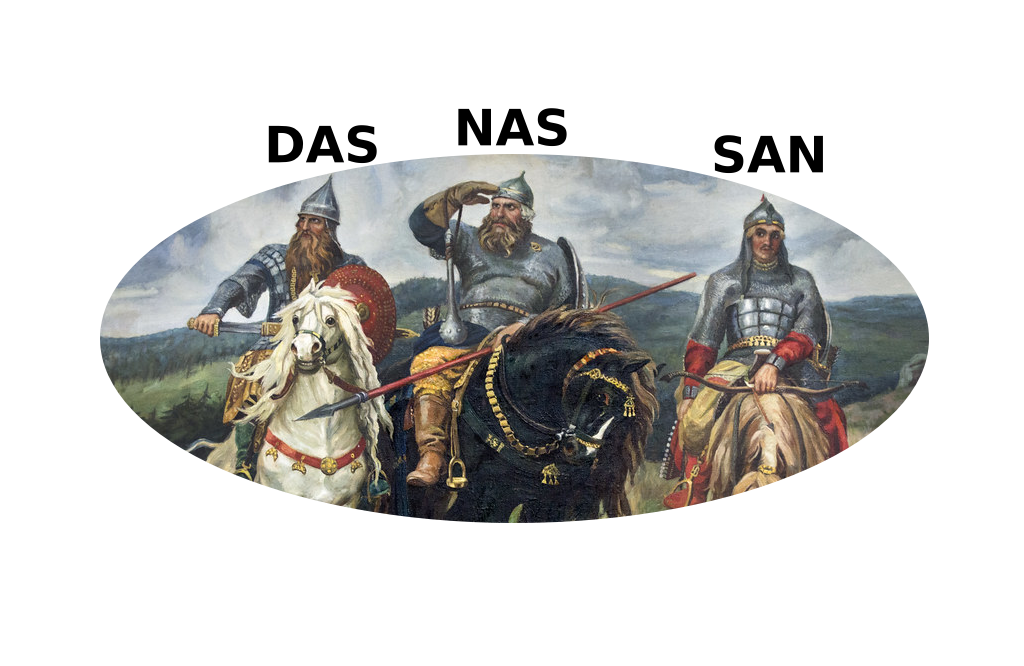
\includegraphics[scale=1.3]{fig/2.tri.png}
\end{frame}

\begin{frame}{Прямое подключение (DAS)}
\begin{columns}[T]
    \begin{column}{.2\textwidth}
        DAS --- directly attached storage
        \dma
    \end{column}
    \begin{column}{.3\textwidth}
    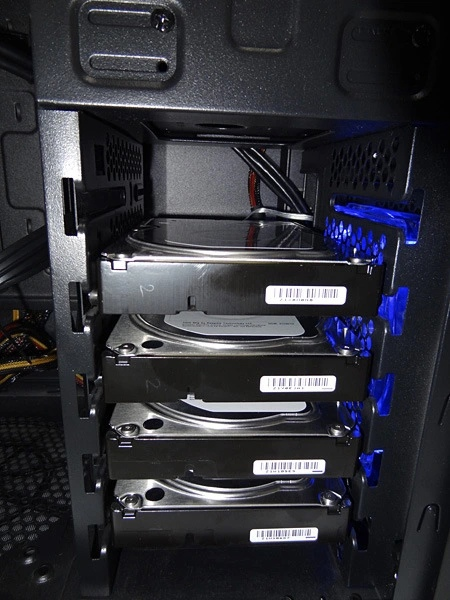
\includegraphics[scale=0.3]{fig/3.hdd.jpg}
    \end{column}
    \begin{column}{.4\textwidth}
        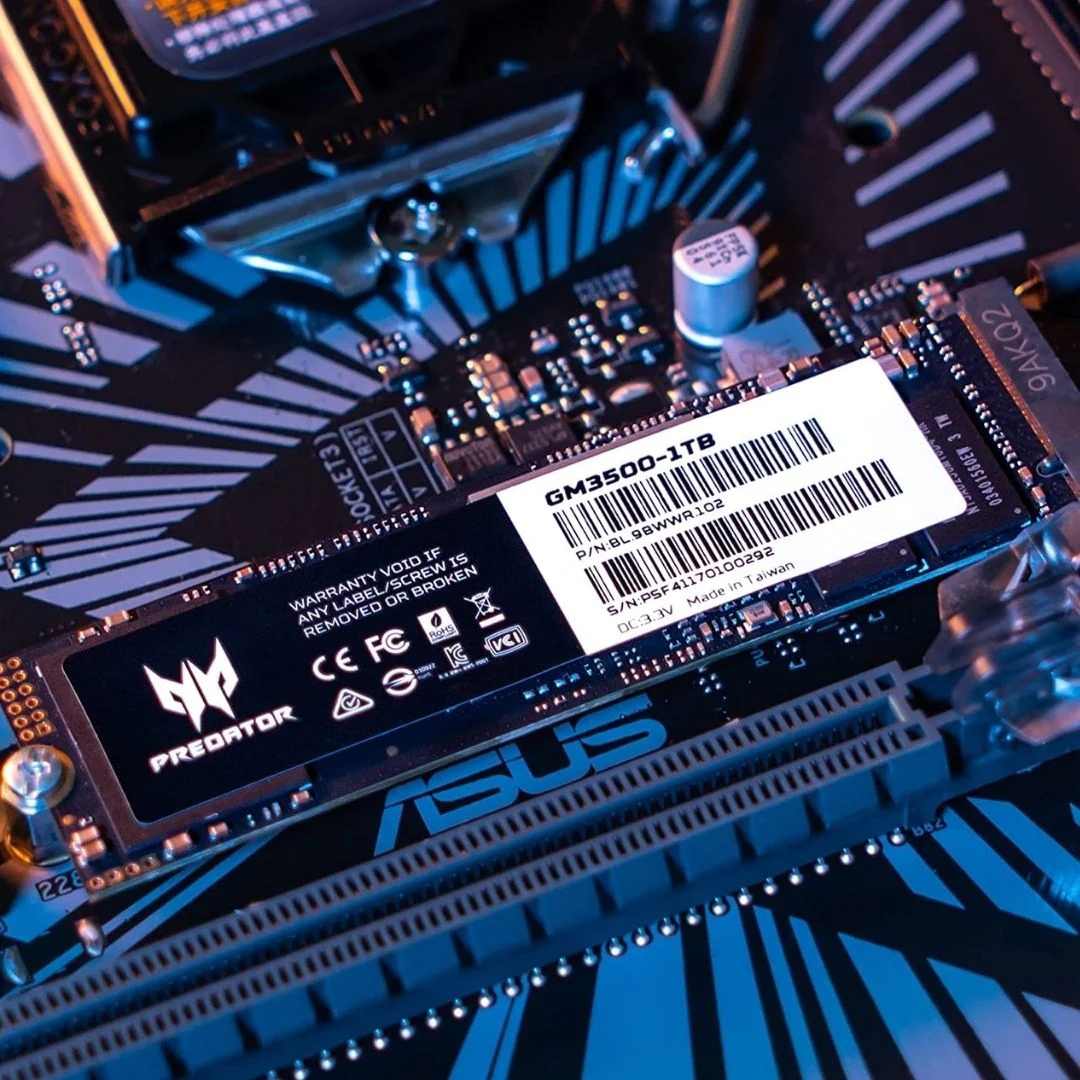
\includegraphics[scale=0.166]{fig/4.nvme.jpg}
    \end{column}
\end{columns}
\end{frame}

\begin{frame}{Подключение по сети (NAS)}
\begin{columns}[T]
    \begin{column}{.4\textwidth}
        NAS --- network attached storage

        В домашнем использовании
        \begin{itemize}
            \item Несколько файловых систем разного типа или с полнодисковым шифрованием
            \item Обход ограничения материнских плат по числу дисков
        \end{itemize}

        В промышленном использовании
        \begin{itemize}
            \item Видеонаблюдение
            \item Сбор информации с датчиков (напр. для автопилота)
        \end{itemize}
    \end{column}
    \hfill
    \begin{column}{.55\textwidth}
        \centering
        \nas
        \vspace{0.7em}
        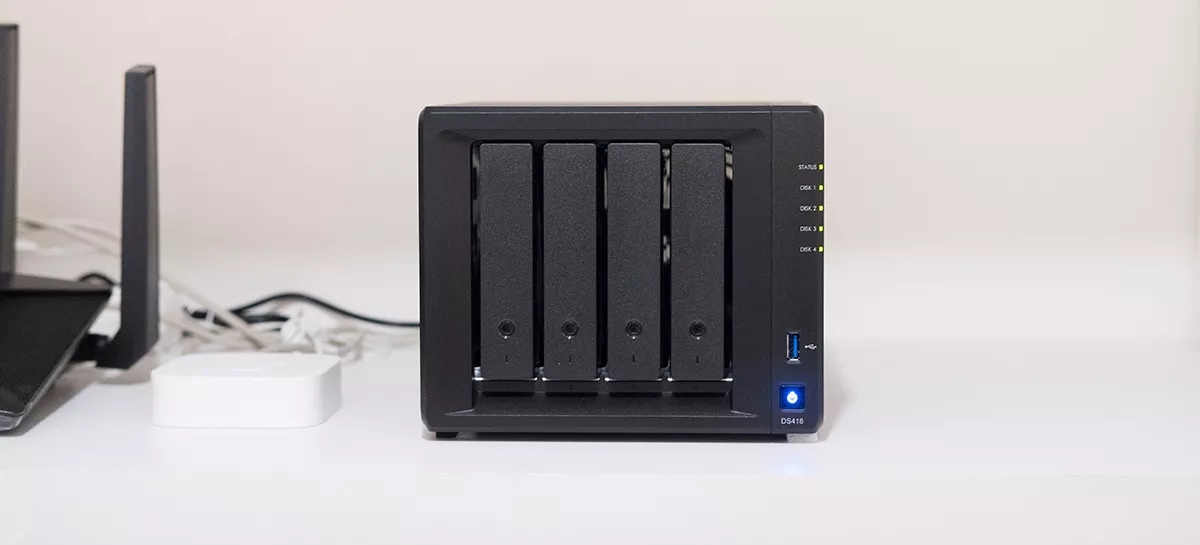
\includegraphics[scale = 0.15]{fig/5.nas.jpg}
    \end{column}
\end{columns}
\end{frame}

\begin{frame}{Сеть хранения данных (SAN)}
\begin{columns}
    \begin{column}{.3\textwidth}
        SAN --- storage area network
        
        \vspace{1em}
        Прежде всего это именно сетевое ПО

        \vspace{1em}
        Примеры функциональности
        \begin{itemize}
            \item Маршрутизация
            \item Аварийное переключение (failover)
            \item Репликация
        \end{itemize}
    \end{column}
    \hfill
    \begin{column}{.66\textwidth}
        \san
    \end{column}
\end{columns}
\end{frame}

\begin{frame}{Аппаратное обеспечение сервера хранения данных}
\begin{columns}
    \begin{column}{.35\textwidth}
        \begin{itemize}
            \item Дополнительные возможности подключения
            \vspace{-1em}
            \begin{itemize}
                \item Для сетевых карт
                \item Для дисков
            \end{itemize}
            \item Быстрая замена накопителей без разбора сервера и отключения питания
            \item Несколько сокетов для процессоров
            \item Несколько блоков питания с возможностью быстрой замены
        \end{itemize}
    \end{column}
    \begin{column}{.6\textwidth}
        \centering
        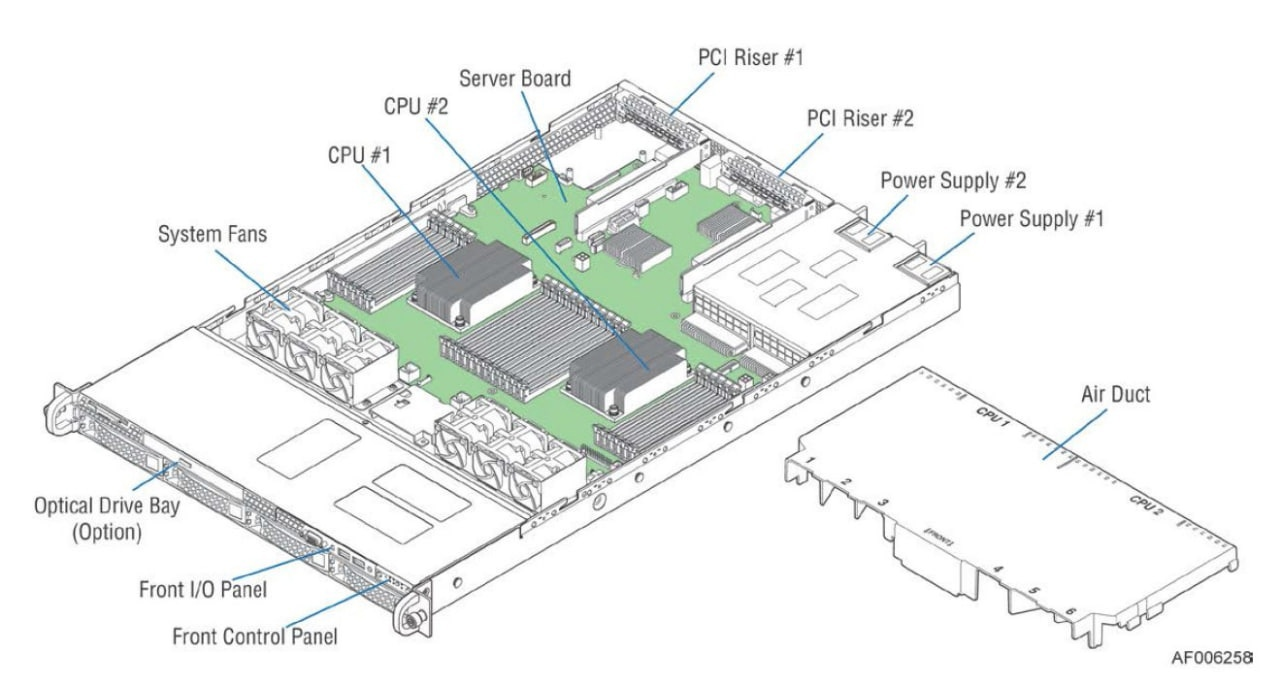
\includegraphics[scale=0.2]{fig/8.server.jpg}
        \tiny Источник: Intel® Server System R1000WT Product Family. Intel® Storage System R1000WT Family. Technical Product Specification
    \end{column}
\end{columns}
\end{frame}

\section{Производительность}

\begin{frame}{RAID для ускорения операций}
    \raidPerf
\end{frame}

\begin{frame}{Бутылочное горлышко --- от CPU к CPU}
    \bottleneck
\end{frame}

\begin{frame}{Software vs. Hardware}
\begin{columns}[T] % align columns
    \begin{column}{.48\textwidth}
    \color{red}\rule{\linewidth}{4pt}
    
    Software
    \begin{itemize}
        \item[+] Оптимизация блочных операций (кэширование, тиринг, QoS, объединение)
        \item[+] Удобное управление
        \item[+] Возможность обновления и добавления функциональности
        \item[+] Разработка ПО на С
        \item[---] Занимает ресурсы CPU
        \item[---] Привязан к ОС

    \end{itemize}
    \end{column}%
    \hfill%
    \begin{column}{.48\textwidth}
    \color{blue}\rule{\linewidth}{4pt}
    
    Hardware
    \begin{itemize}
        \item[+] Позволяет начинать операции до загрузки ОС
        \item[+] Встроенный UPS 
        \item[---] Занимает PCIe слот
        \item[---] Невозможность обновлений
        \item[---] Для настройки требуется выключать сервер
        \item[---] Сложно разрабатывать ПО
    \end{itemize} 
    \end{column}%

\end{columns}
\vspace{1em}
    \let\thefootnote\relax\footnotetext{\fontsize{7}{8}\selectfont Важно отметить, что на вопрос о производительности “дискуссионный”. Если просто ввести запрос в гугл, то можно найти множество статей, утверждающих, что hardware быстрее, но дороже. Это устаревшая информация, не верьте ей. Hardware рейды до сих пор используются, но скорее маленькими компаниями для внутренних нужд. Например у Dell (\url{https://www.dell.com/en-us/shop/scc/sc/storage-products#portfolio}) сервера в основном с software рейдом}
\end{frame}

\begin{frame}{Об оптимизациях}
    \centering
    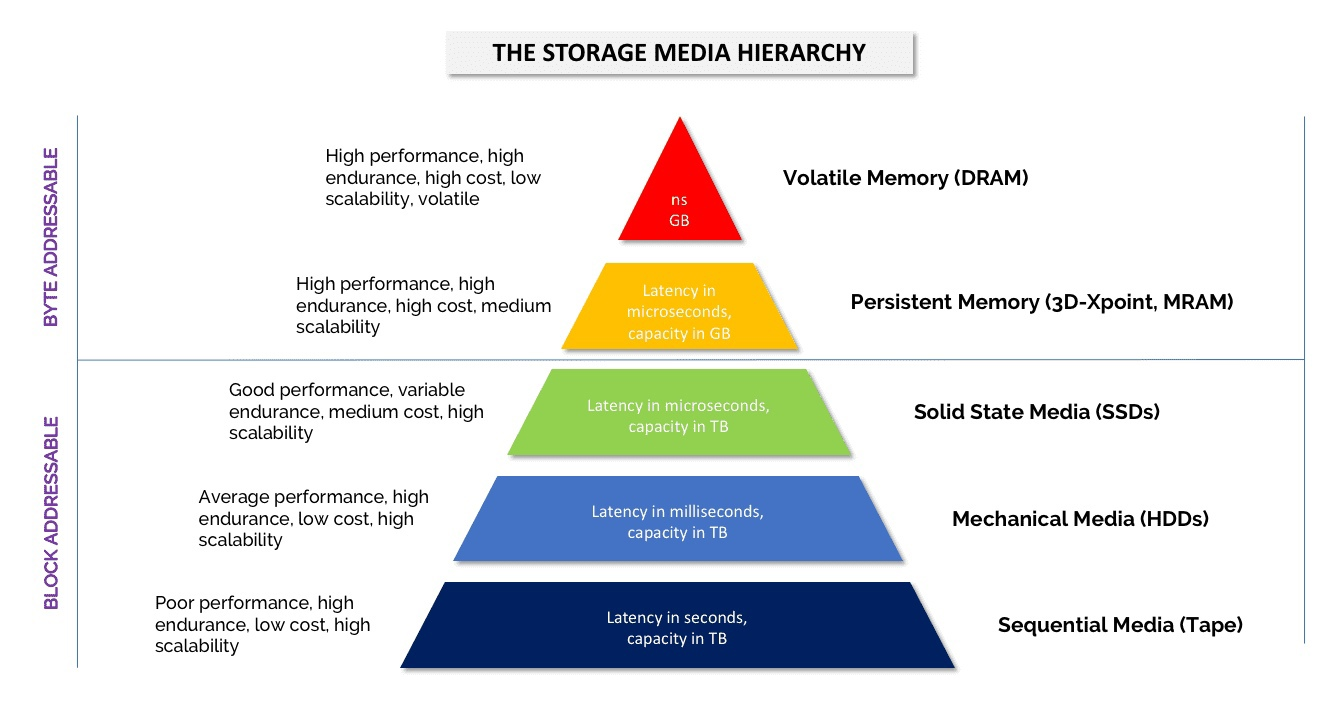
\includegraphics[scale=0.25]{fig/9.tiering.jpg}
    
    \tiny Источник: \url{https://www.architecting.it/blog/caching-tiering/}
\end{frame}

\section{Целостность}

\begin{frame}{RAID для надежности}
\raid
\begin{align*}
    RAID\ failure\ rate = f(ndrives, nparity, capacity, drive\ failure\ rate)\footnotemark
\end{align*}
\footnotetext[1]{\url{https://www.ibm.com/support/pages/re-evaluating-raid-5-and-raid-6-slower-larger-drives}}
\end{frame}

\begin{frame}{Математика RAID-массива}
    \begin{itemize}
        \item XOR
        \begin{itemize}
            \item RAID 5
            \item Исправляют одну ошибку
        \end{itemize}
        \item Коды Хэмминга
        \begin{itemize}
            \item RAID 2
            \item Из $(2^n - 1)$ дисков $n$ дисков под коды
            \item Исправляет одну ошибку, обнаруживает двойную ошибку 
        \end{itemize}
        \item Коды Рида-Соломона
        \begin{itemize}
            \item RAID 6, исправляет 2 ошибки
            \item RAID N+M, исправляет M ошибок
        \end{itemize}
    \end{itemize}
\end{frame}

\begin{frame}{Коды Рида-Соломона}
\stripe

    \begin{minipage}{.48\textwidth}
        Вычисление P, Q (encode)
    \end{minipage}
    \begin{minipage}{.48\textwidth}
        Восстановление данных (decode)
    \end{minipage}

\begin{columns}[T]
    \begin{column}{.48\textwidth}
    \begin{minipage}[t][.5\textheight][t]{\textwidth}
        \begin{align*}
            P &= \sum_{i=0}^{N-1} D_i \\
            Q &= \sum_{i=0}^{N-1} q_i D_i
        \end{align*}
    \end{minipage}
    \end{column}

    
    \begin{column}{.48\textwidth}
    \begin{minipage}[t][.5\textheight][t]{\textwidth}
        \only<1>{
        \begin{align*}
            D_\alpha + D_\beta &= P - \sum_{i=0}^{N-1} D_i & i \neq \alpha, \beta \\
            q_\alpha D_\alpha + q_\beta D_\beta &= Q - \sum_{i=0}^{N-1} q_i D_i & i \neq \alpha, \beta 
        \end{align*}
        }
        \only<2>{
        \begin{align*}
            D_\alpha + D_\beta &= \bar{P}_{\alpha, \beta} \\
            q_\alpha D_\alpha + q_\beta D_\beta &= \bar{Q}_{\alpha, \beta}
        \end{align*}
        }

        \only<3>{
        \begin{align*}
            D_\alpha &= \bar{P}_{\alpha, \beta} - D_\beta \\
            q_\alpha D_\alpha + q_\beta D_\beta &= \bar{Q}_{\alpha, \beta}
        \end{align*}
        }
        
        \only<4>{
        \begin{align*}
            D_\alpha &= \bar{P}_{\alpha, \beta} - D_\beta \\
            q_\alpha (\bar{P}_{\alpha, \beta} - D_\beta) + q_\beta D_\beta &= \bar{Q}_{\alpha, \beta}
        \end{align*}
        }

        \onslide<5->{
        \begin{align*}
            D_\alpha &= \bar{P}_{\alpha, \beta} - D_\beta \\
            (q_\beta - q_\alpha) D_\beta &= \bar{Q}_{\alpha, \beta} - \bar{P}_{\alpha, \beta} q_\alpha
        \end{align*}
        }

        % \onslide<6->{
        % \begin{align*}
        %     D_\alpha &= \bar{P}_{\alpha, \beta} - D_\beta \\
        %     (q_\beta - q_\alpha) D_\beta &= \bar{Q}_{\alpha, \beta} - \bar{P}_{\alpha, \beta} q_\alpha
        % \end{align*}
        % }

        \vspace{-2em}
        \begin{itemize}
            \item<6-> $q_\beta \neq q_\alpha$ 
            \item<7-> $q_\beta - q_\alpha$ обратим
            \item<8-> Конечные поля!
        \end{itemize}

        \end{minipage}
    \end{column}
\end{columns}

\let\thefootnote\relax\footnotetext{Федоров А. Р. Способы кодирования информации для построения программных отказоустойчивых дисковых массивов (\url{https://www.elibrary.ru/item.asp?id=20262093})}

\end{frame}

\begin{frame}{RAID 6. Запись}
Аналогично RAID 5 при записи данных надо также вычислить и записать контрольно-восстановительные суммы (P и Q)
\begin{enumerate}
    \item Вычисление P и Q через Encode
    \begin{itemize}
        \item Требуется одинаковый кусок данных с каждого диска
        \item Чтение с дисков, не участвующих в операции (на которых не будет записи)
        \item Особенно неэффективно для небольших запросов (напр. 4 KiB)
        \item Может выполнятся в несогласованном состоянии данных и синдромов
    \end{itemize}
    \item Вычисление P и Q через Update
    \begin{itemize}
        \item Для вычисления нужно прочитать только старые данные и старые синдромы (те же части, которые будут записаны)    
        \item В некоторых случаях может быть медленнее, чем через encode
        \item Не может быть выполнено в несогласованном состоянии данных и синдромов, для того, чтобы выполнять такие операции после создания RAID нужно посчитать и записать все контрольно-восстановительные суммы (процесс инициализации)
    \end{itemize}
\end{enumerate}
\end{frame}

\begin{frame}{RAID 6. Запись. Write hole}
    Записи на каждый диск выполняются независимо. Если происходит отключение питания, то могло записаться разное количество данных на каждом из дисков и может возникнуть несогласованном состоянии данных и синдромов, в таком случае нельзя делать запись через update
    \begin{columns}
        \begin{column}{.54\textwidth}
            \writehole
        \end{column}
        \begin{column}{.42\textwidth}
        
        \vspace{1em}
        Пути решения проблемы
            \begin{itemize}
                \item Единственный бит в метаданных на весь рейд, по которому можно определить, был ли он выгружен корректно
                \item Битовая карта последних записей
                \item Журнал
            \end{itemize}
        \end{column}
    \end{columns}
    
\end{frame}

\end{document}
